% Talk (10--15 min) on Finzi et al., "From Entropy to Epiplexity", arXiv:2601.03220v2, 16 March 2026 (latest version).
% figs/ holds the vector figures of the arXiv v2 source (byte-identical to v1), unchanged; slides crop them with `trim'.
% Statement and figure numbers ("Thm. 9 of the paper", "Fig. 3") follow v2; v2 kept the v1 numbering.
% Build (twice): pdflatex epiplexity_talk.tex
% Audience questions include their answers on slide 17.
\documentclass[aspectratio=169,notheorems]{beamer}
\usetheme{default}
\usefonttheme{professionalfonts}
\setbeamersize{text margin left=8mm,text margin right=8mm}
\setbeamertemplate{navigation symbols}{}
\setbeamertemplate{footline}[frame number]
\setbeamertemplate{itemize item}{--}
\setbeamertemplate{itemize subitem}{--}
\usepackage[T1]{fontenc}
\usepackage{lmodern}
\usepackage{amsmath,amssymb,mathtools,booktabs,array}
\usepackage{microtype}
\usepackage{natbib}
\renewcommand{\bibsection}{}
\definecolor{myblue}{RGB}{25,75,130}
\setbeamercolor{structure}{fg=myblue}
\setbeamercolor{frametitle}{fg=myblue}
\setbeamerfont{frametitle}{size=\large,series=\bfseries}
\setbeamertemplate{blocks}[rounded][shadow=false]
\setbeamercolor{block title}{fg=myblue,bg=myblue!12}
\setbeamercolor{block body}{bg=myblue!4}
\setbeamertemplate{theorems}[numbered]
% one counter per kind; upright bodies
\theoremstyle{definition}
\newtheorem{definition}{Definition}
\newtheorem{theorem}{Theorem}
\newtheorem{proposition}{Proposition}
\newcommand{\E}{\mathbb{E}}
\newcommand{\KL}{\mathrm{KL}}
\newcommand{\MDL}{\mathrm{MDL}}
\newcommand{\Dt}{\mathcal{D}}
\newcommand{\PT}{\mathcal{P}_T}
\newcommand{\Poly}{\mathrm{Poly}}
\newcommand{\prog}{\mathrm{P}}
\DeclareMathOperator*{\argmin}{arg\,min}
% the claim a slide closes on
\newcommand{\take}[1]{\par\vspace{0.35em}{\color{myblue}\hrule height 0.6pt}\vspace{0.25em}\noindent\textbf{#1}\par}
% one sentence of provenance under a figure
\newcommand{\src}[1]{{\scriptsize\color{black!60}#1\par}}

\begin{document}
% ============================================================ TITLE
\begin{frame}[plain]
\centering
\vspace*{1.2em}
{\LARGE\bfseries\color{myblue} From Entropy to Epiplexity}\\[0.5em]
{\large Rethinking Information for Computationally Bounded Intelligence}\\[1.8em]
Marc Finzi, Shikai Qiu, Yiding Jiang, Pavel Izmailov, J.~Zico Kolter, Andrew Gordon Wilson\\[0.2em]
{\small Carnegie Mellon University, New York University}\\[0.2em]
{\small arXiv:2601.03220, version~2, 16 March 2026}\\[2.2em]
Speaker: Alex Kravatsky
\end{frame}
% ============================================================ MOTIVATION
\begin{frame}{Which pretraining data support transfer?}
\begin{columns}[T]
\begin{column}{0.54\textwidth}
\begin{itemize}\setlength{\itemsep}{0.7em}
\item Models pretrained on text can improve performance on robotics, theorem proving and forecasting tasks.
\item Dataset size alone does not measure reusable predictive structure.
\item \textbf{Question:} how much structure can a particular learner extract, given a fixed compute budget?
\end{itemize}
\end{column}
\begin{column}{0.42\textwidth}
\centering
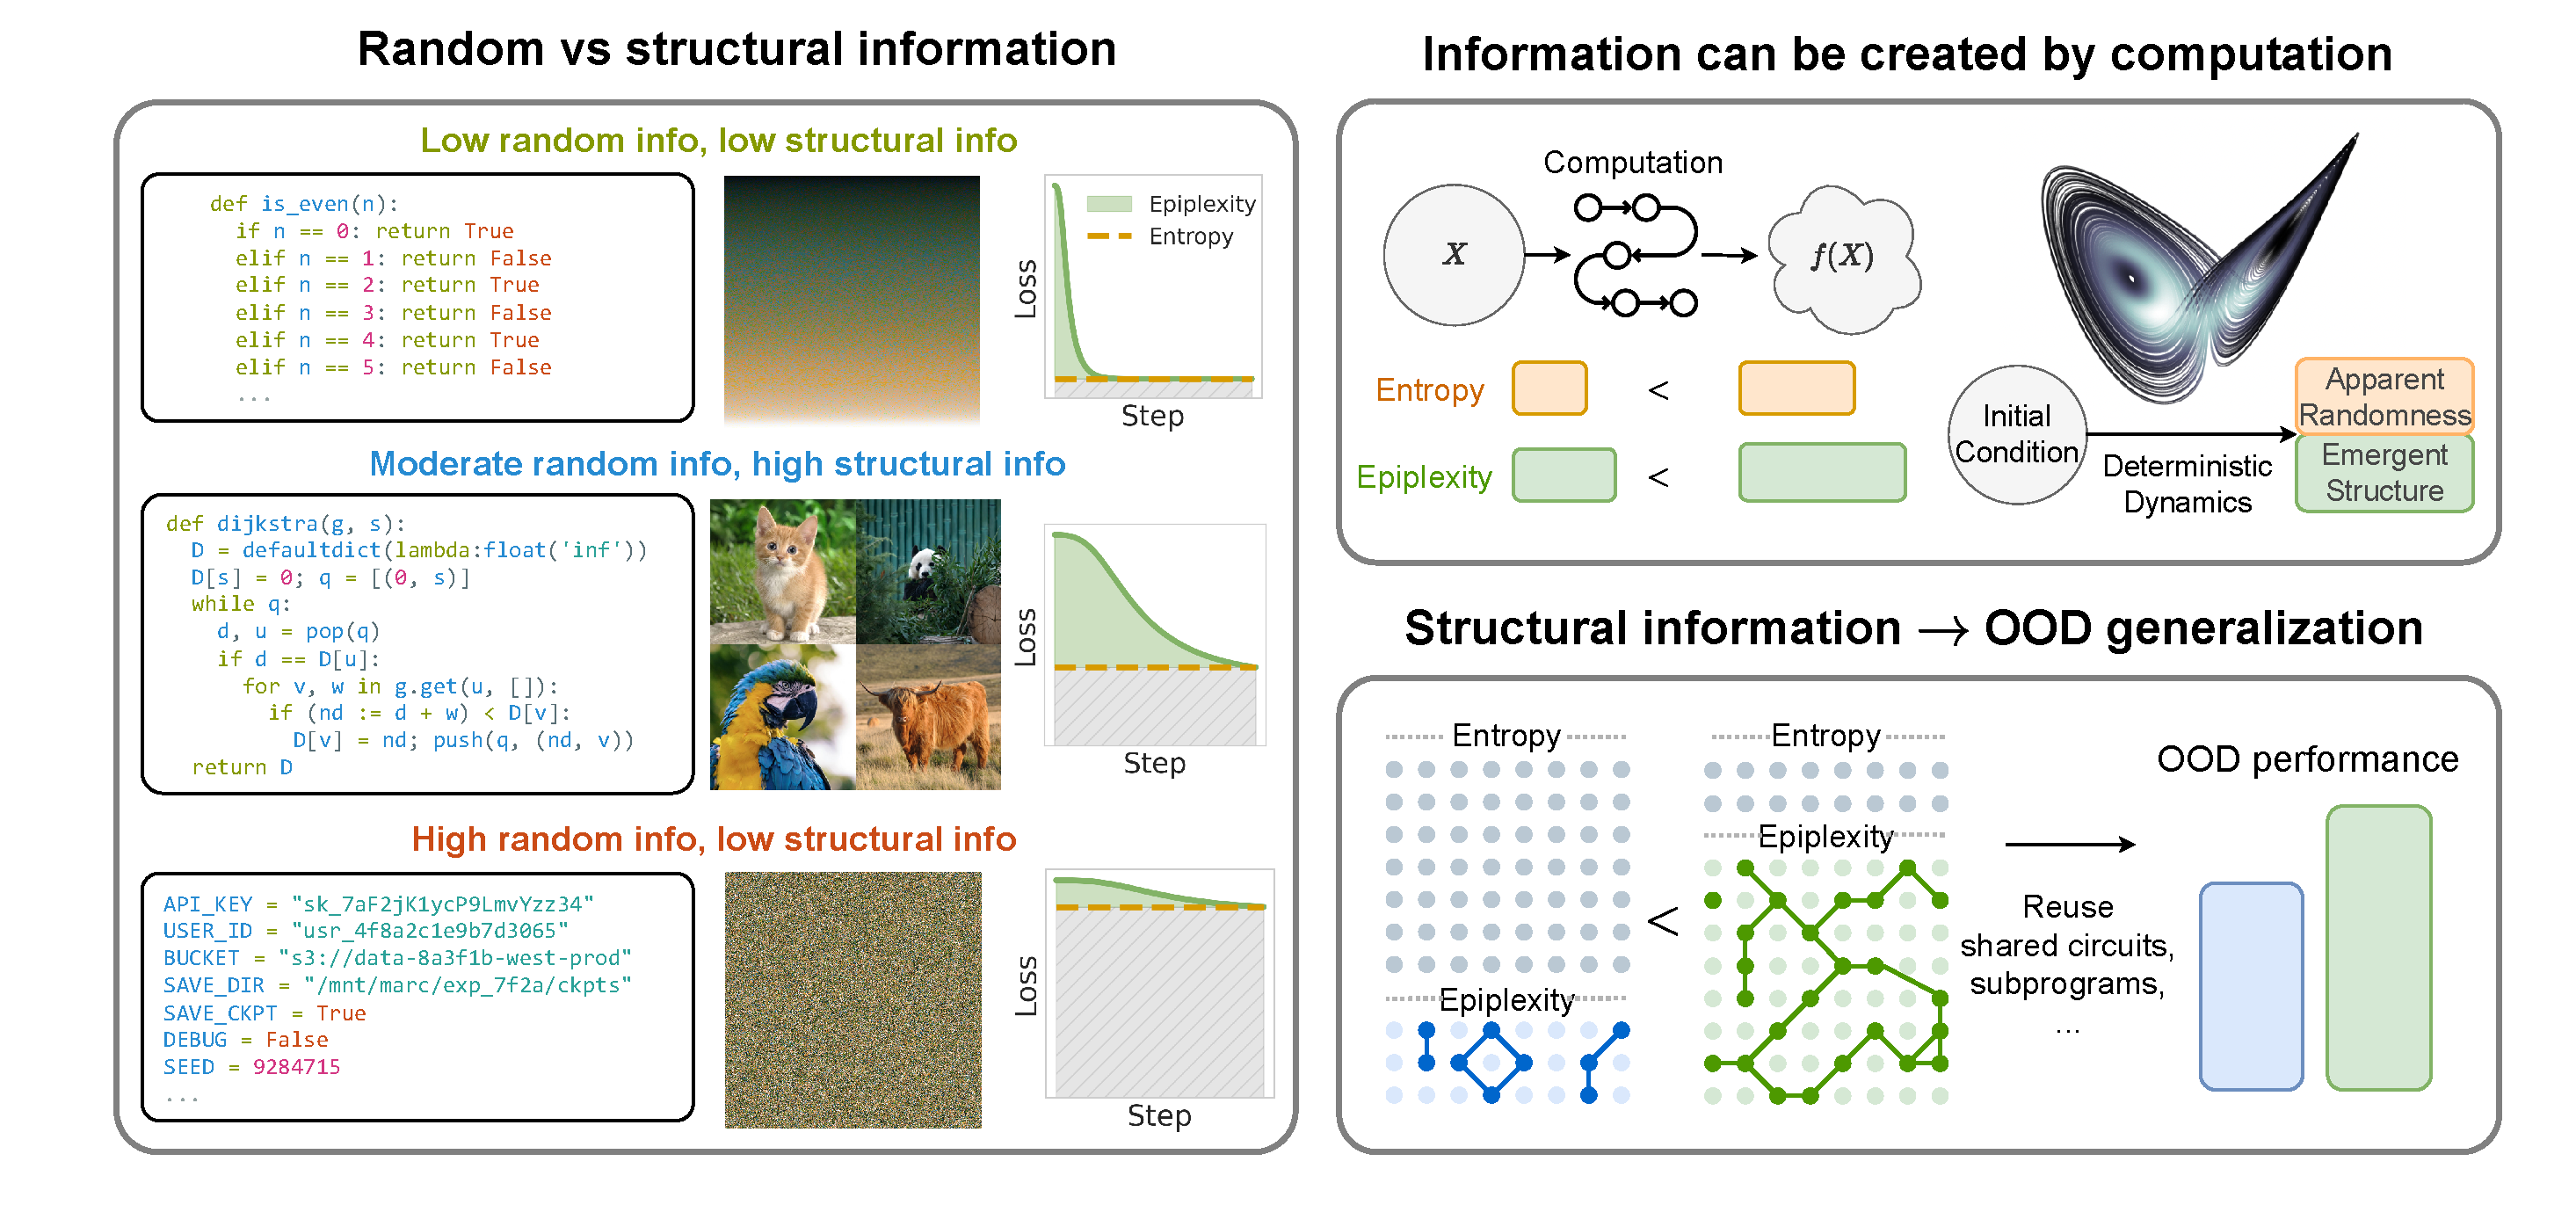
\includegraphics[width=\linewidth,trim=0 0 660 40,clip]{figs/fig1.pdf}
\raggedright
\src{Training loss on three kinds of data. Dashed line: final loss; green area: loss removed by learning. Source: Fig.~1 of \citet{finzi2026}.}
\end{column}
\end{columns}
\end{frame}
% ------------------------------------------------------------
\begin{frame}{Two classical lenses on information}
\small
$H(X)=\E[-\log_2 p(X)]$ is the Shannon entropy of a random variable $X$ with probability mass function $p$.
It is the ideal average code length in bits for a draw from the distribution.

\medskip
$K(x)$ is the Kolmogorov complexity of one realised string $x$: the length of the shortest self-delimiting program that outputs
$x$ on a fixed universal computer $\mathcal U$ \citep{livitanyi2008}.

\smallskip
\renewcommand{\arraystretch}{1.15}
\begin{tabular}{@{}>{\raggedright\arraybackslash}p{0.49\textwidth}>{\raggedright\arraybackslash}p{0.47\textwidth}@{}}
\toprule
\textbf{Shannon entropy} & \textbf{Kolmogorov complexity} \\
\midrule
Uncertainty in a distribution. Uniform $n$-bit strings have entropy $n$; a distribution concentrated on one string has entropy zero. &
Program length for one string. A repeating pattern can be specified by its rule and length; a typical random string needs about $n$ bits. \\
\bottomrule
\end{tabular}
\smallskip
Kolmogorov complexity is a mathematical benchmark; no algorithm computes $K(x)$ exactly for every string.
\normalsize
\take{Entropy measures average uncertainty; Kolmogorov complexity measures program length.}
\end{frame}
% ============================================================ FORMAL PROBLEM STATEMENT
\begin{frame}{The missing ingredient: computational access}
\small
Neither classical quantity asks whether a learner can find or use the relevant pattern within a finite budget.
For example, a deterministic training run can produce a network with useful circuits, although the rules and
random seed form a short description of the run.

\medskip
\begin{itemize}\setlength{\itemsep}{0.35em}
\item A weak observer may treat a structured process as random.
\item A stronger observer may discover a compact predictive model.
\item We therefore define information relative to the models available within time $T$.
\end{itemize}

\take{Epiplexity measures model bits in the best description available under a time bound.}
\end{frame}
% ------------------------------------------------------------
\begin{frame}{A model with bounded computation}
\small
Fix a prefix-free universal computer $\mathcal U$ and a time bound $T(n)$. The observer may use only
programs $\prog\in\PT$ that, within $T(n)$ steps, can both
\begin{itemize}\setlength{\itemsep}{0.25em}
\item evaluate a probability $P(x)$ for an observation $x$;
\item sample a new $x$ from the same distribution $P$.
\end{itemize}

\medskip
The program length $|\prog|$ is measured in bits. This is the idealised definition; in experiments we
replace $\PT$ by models reachable with a stated architecture, optimiser and FLOP budget.

\medskip
\take{The formal bound limits evaluation and sampling; empirical estimates also account for training.}
\end{frame}
% ------------------------------------------------------------
\begin{frame}{Epiplexity: the two-part description}
\begin{definition}[Def.~8 of the paper]\label{def:epi}
For a random variable $X$ on $\{0,1\}^n$, let
\vspace{-0.4em}
\[
\prog^\star=\argmin_{\prog\in\PT}\bigl\{|\prog|+\E[-\log P(X)]\bigr\},
\]
with ties broken by the shortest program. Logarithms are base~$2$. The \emph{epiplexity} of $X$ is $S_T(X):=|\prog^\star|$. The \emph{time-bounded entropy} of $X$ is $H_T(X):=\E[-\log P^\star(X)]$.
\end{definition}
\small
$S_T$ is the model part: bits needed to describe the selected predictor. $H_T$ is the data part: expected bits
needed to encode data with that predictor. Their sum $\MDL_T(X):=S_T(X)+H_T(X)$ is the minimum two-part
description length under the bound.

\smallskip
\centering
\begin{tabular}{@{}llcc@{}}
\toprule
Random variable $X$ & Time bound & $S_T(X)$ & $H_T(X)$ \\
\midrule
$U_n$, uniform on $\{0,1\}^n$ & enough for uniform model & $O(1)$ & $n+O(1)$ \\
$0101\ldots$ or $1010\ldots$, probability $\tfrac12$ each & $T(n)=\Theta(n)$ & $O(1)$ & $O(1)$ \\
\bottomrule
\end{tabular}

\smallskip
\raggedright
For $U_n$, $S_T=O(1)$ and $H_T\ge n$. For the alternating pair, both parts are $O(1)$.
\end{frame}
% ============================================================ THEORY
\begin{frame}{Two consequences of the time bound}
\small
\begin{itemize}\setlength{\itemsep}{0.65em}
\item \textbf{Pseudorandom generator.} A short seed is stretched into $n$ bits. Shannon entropy sees
      only the seed; a polynomial-time observer sees almost $n$ unpredictable bits and almost no structure.
\item \textbf{One-way map.} For $Y=f(X)$, predicting $Y$ from $X$ is easy, while recovering $X$ from
      $Y$ is hard. A bounded observer assigns different information to the two orders.
\end{itemize}

\medskip
For supervised learning we use the conditional version $S_T(Y\mid X)$: the input $X$ is available,
and only the labels $Y$ are encoded.

\medskip
\take{The same data can look random or structured depending on what the observer can compute.}
\end{frame}
% ============================================================ METHOD
\begin{frame}{From programs to networks: the compute-optimal code}
\begin{columns}[T]
\begin{column}{0.58\textwidth}
\small
\begin{itemize}\setlength{\itemsep}{0.25em}
\item Search over all programs is intractable, so fix an architecture and optimiser.
\item Approximate dense-model accounting: $6ND+2N\Dt\le T$, where $N$ counts parameters and $D,\Dt$ count training and evaluation tokens.
\item Each run gives a model code plus a validation-data code. Select the shortest admissible two-part code; a lower hull smooths the empirical curve.
\item Report its model and data parts as estimates $\widehat S_T$ and $\widehat H_T$.
\end{itemize}
\end{column}
\begin{column}{0.38\textwidth}
\vspace{0.5em}
\centering
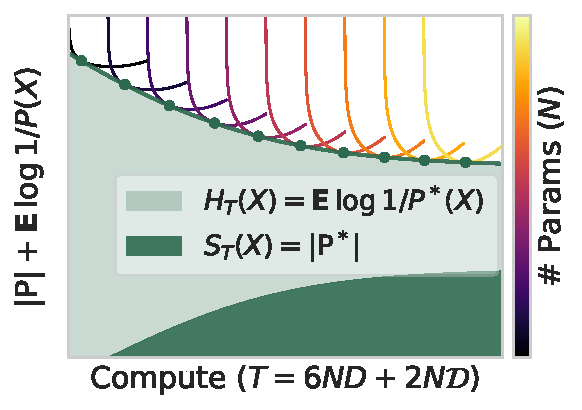
\includegraphics[width=\linewidth]{figs/pareto_frontier.pdf}
\raggedright
\src{Schematic. Thin curves: training runs, coloured by $N$. Dots: the lower envelope. Dark green: $S_T$; light green: $H_T$. Source: Fig.~2b of \citet{finzi2026}.}
\end{column}
\end{columns}
\end{frame}
% ------------------------------------------------------------
\begin{frame}{Estimation I: the prequential code}
\begin{columns}[T]
\begin{column}{0.64\textwidth}
\small
\begin{itemize}\setlength{\itemsep}{0.2em}
\item $P_i$ has seen $Z_0,\ldots,Z_{i-1}$; $P_0$ is the initial model.
\item Encode $Z_i$ at ideal cost $-\log_2P_i(Z_i)$, then update. The decoder repeats the update.
\item The sequential data code sums these costs. Subtract the final-model data code to estimate the model part:
\[
\widehat K_{\mathrm{preq}}=\sum_{i<M}\bigl[-\log P_i(Z_i)+\log P_M(Z_i)\bigr].
\]
\end{itemize}
\end{column}
\begin{column}{0.32\textwidth}
\vspace{0.5em}
\centering
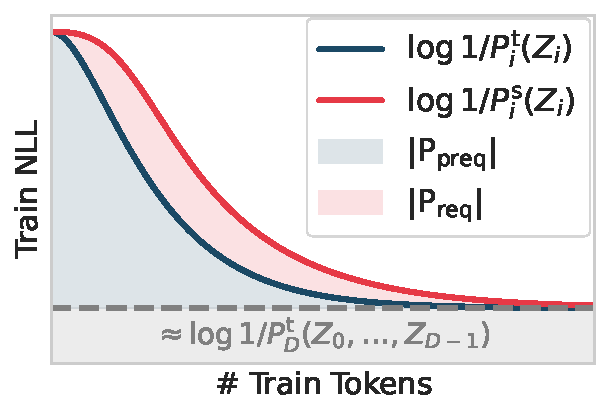
\includegraphics[width=\linewidth]{figs/requential_illustration.pdf}
\raggedright
\src{Dark curve: $\log 1/P_i(Z_i)$ of the network trained on real data (superscript t). Blue area: $|\prog_{\mathrm{preq}}|$. Red curve and red area: the requential code of the next slide. Source: Fig.~2a of \citet{finzi2026}.}
\end{column}
\end{columns}
\small
\begin{itemize}\setlength{\itemsep}{0.2em}
\item The loss is measured before fitting each example, so it is a test-like loss.
\item The area is a heuristic model-part estimate; subtraction alone gives no model-only code.
\end{itemize}
\end{frame}
% ------------------------------------------------------------
\begin{frame}{Estimation II: the requential code}
\small
\begin{itemize}\setlength{\itemsep}{0.25em}
\item A teacher model trains on real data; a student model trains on teacher-distributed samples \citep{qiu2026}.
\item Both sides share the student and a random seed. Send the index of a student proposal selected to have the teacher's distribution.
\item Relative entropy coding bounds the expected message cost by teacher--student disagreement:
\[
\E[\ell_i\mid\mathcal F_i]\le\KL_i+2\log(1+\KL_i)+\kappa,\quad \kappa<5.21,
\]
where $\KL_i=\KL(P_i^{\mathrm t}\Vert P_i^{\mathrm s})$ and $\mathcal F_i$ is the prior history. Summing gives the student-code bound; $\sum_i\KL_i$ is its leading estimate.
\end{itemize}
\centering
\begin{tabular}{@{}lll@{}}
\toprule
& Prequential & Requential \\
\midrule
Model part & heuristic subtraction & explicit student reconstruction \\
Training & one network & teacher and student, $2$--$10\times$ slower \\
Reported values & larger in the paper & smaller in the paper \\
\bottomrule
\end{tabular}
\raggedright
\take{Prequential is cheaper; requential has an explicit code.}
\end{frame}
% ============================================================ EXPERIMENTS
\begin{frame}{Experiment: cellular automata create structure}
\small
An \emph{elementary cellular automaton} (ECA) updates binary cells in parallel from their three-cell neighbourhoods \citep{wolfram2002}.\par
\textbf{Setting.} $64$ periodic cells; $Y=F_r^{48}(X)$; transformer sweep; requential code.

\smallskip
\begin{columns}[T]
\begin{column}{0.47\textwidth}
\centering
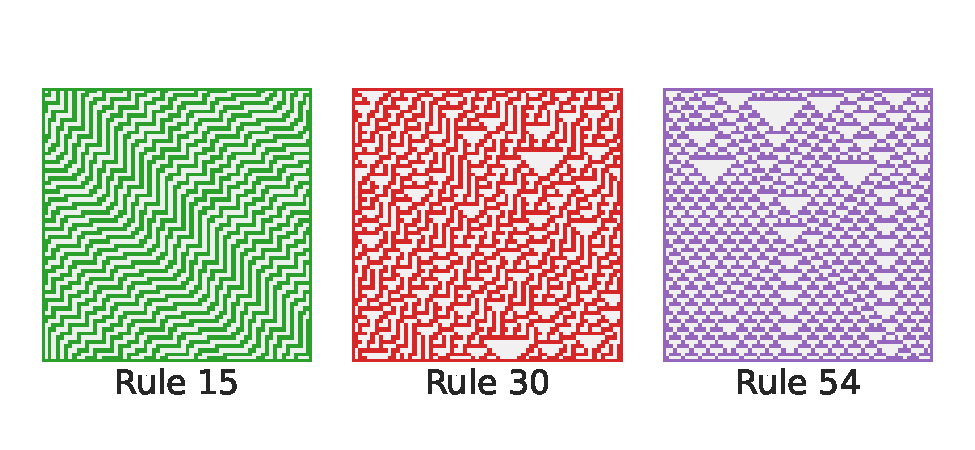
\includegraphics[width=0.72\linewidth,trim=18 19 15 38,clip]{figs/eca_spacetime.pdf}

\smallskip
\begin{tabular}{@{}lccc@{}}
\toprule
Rule & 15 & 30 & 54 \\
\midrule
$S_T(Y\mid X)$, bits & $2\times10^5$ & $\approx0$ & $5.4\times10^6$ \\
$H_T(Y\mid X)$, bits & $\approx0$ & $10^8$ & $1.5\times10^7$ \\
\bottomrule
\end{tabular}
\end{column}
\begin{column}{0.45\textwidth}
\centering
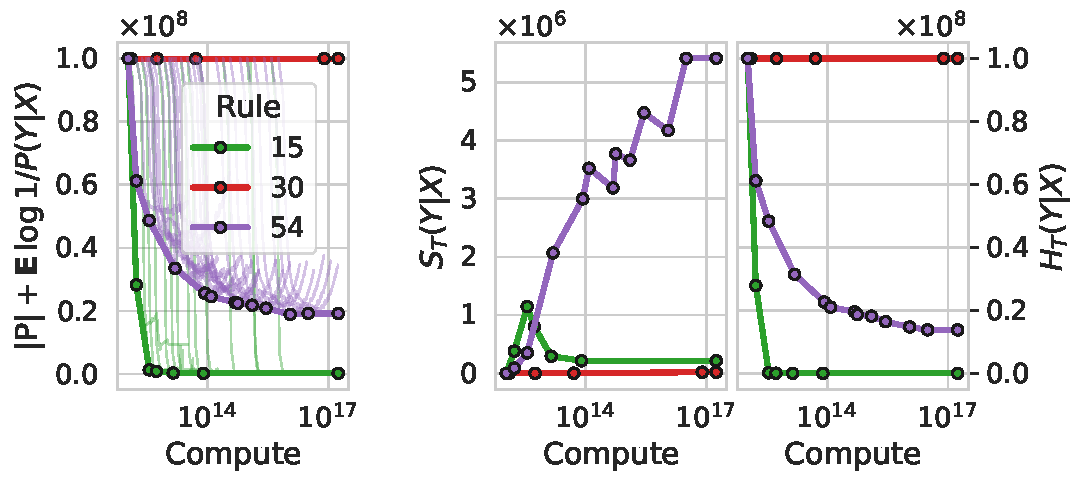
\includegraphics[height=3.6cm,trim=180 0 0 0,clip]{figs/eca_rules_measurements.pdf}
\end{column}
\end{columns}
\src{Left: rollouts, time downward. Right: $S_T$ and $H_T$ against compute in FLOPs. Table: our estimates from the plots at $10^{17}$ FLOPs. Source: Fig.~3 of \citet{finzi2026}.}
\take{Rule 15 is simple, rule 30 looks random, and rule 54 contains learnable structure.}
\end{frame}
% ------------------------------------------------------------
\begin{frame}{Experiment: prediction requires more structure than generation}
\small
\textbf{Setting.} Hide $h$ bits of a random $Z\in\{0,1\}^{32}$; predict four rule~30 updates of $Z$ from the visible bits.

\smallskip
\begin{columns}[c]
\begin{column}{0.4\textwidth}
\centering
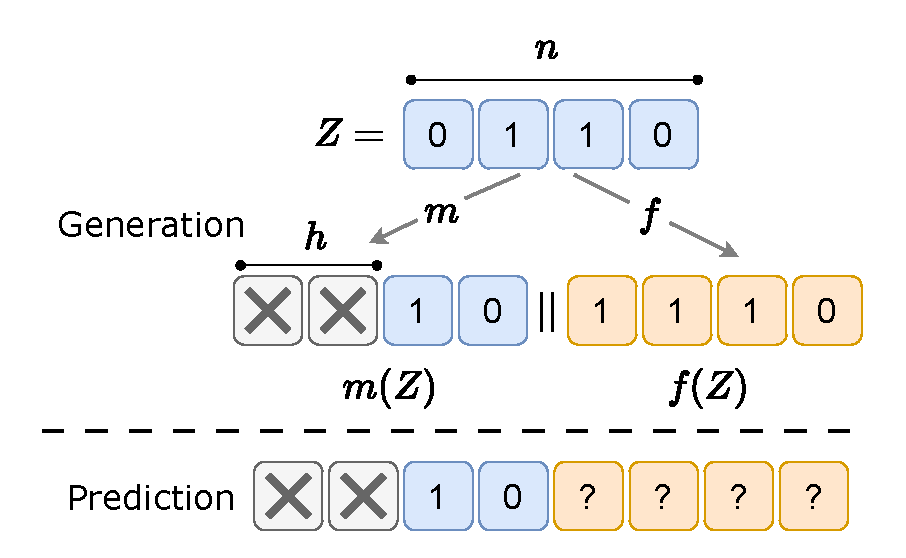
\includegraphics[height=2.6cm]{figs/hidden_bits_illustration.pdf}
\end{column}
\begin{column}{0.5\textwidth}
\centering
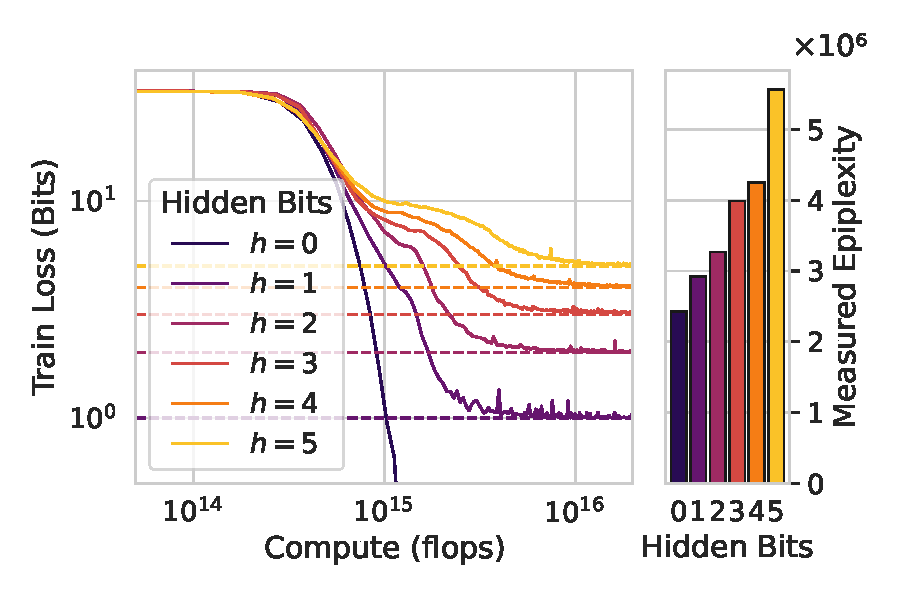
\includegraphics[height=3.1cm]{figs/induction_hard.pdf}
\end{column}
\end{columns}
\src{Left: the data. Right: training loss against compute in FLOPs (dashed: $h$ bits) and $S_T$ for each $h$. Source: Fig.~5 of \citet{finzi2026}.}
\begin{itemize}
\item The generator runs forward; the predictor must infer the hidden bits.
\item The loss approaches $h$ bits only after rapidly growing compute, and $S_T$ grows with $h$.
\end{itemize}
\take{Predicting with partial observations requires inference that is absent from forward generation.}
\end{frame}
% ------------------------------------------------------------
\begin{frame}{Experiment: the order of chess data}
\small
\textbf{Setting.} Lichess games in two orders: moves $\to$ final board, or board $\to$ moves. Transformer sweep with requential coding.

\smallskip
\begin{columns}[c]
\begin{column}{0.44\textwidth}
\centering
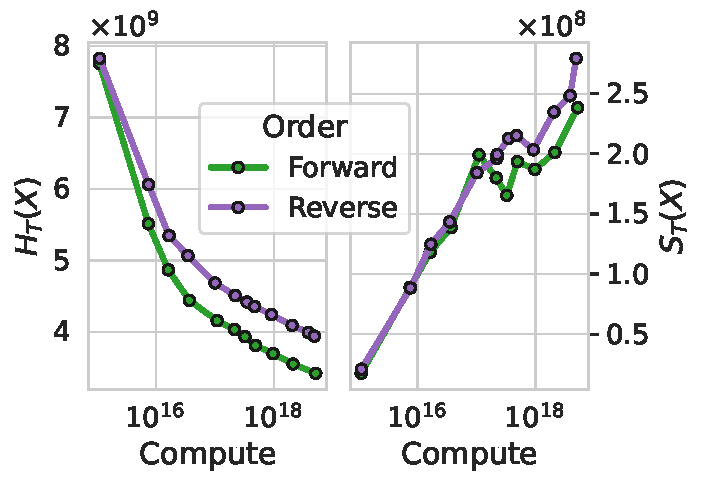
\includegraphics[height=3.0cm]{figs/chess_entropy_and_epi.pdf}
\end{column}
\begin{column}{0.4\textwidth}
\centering
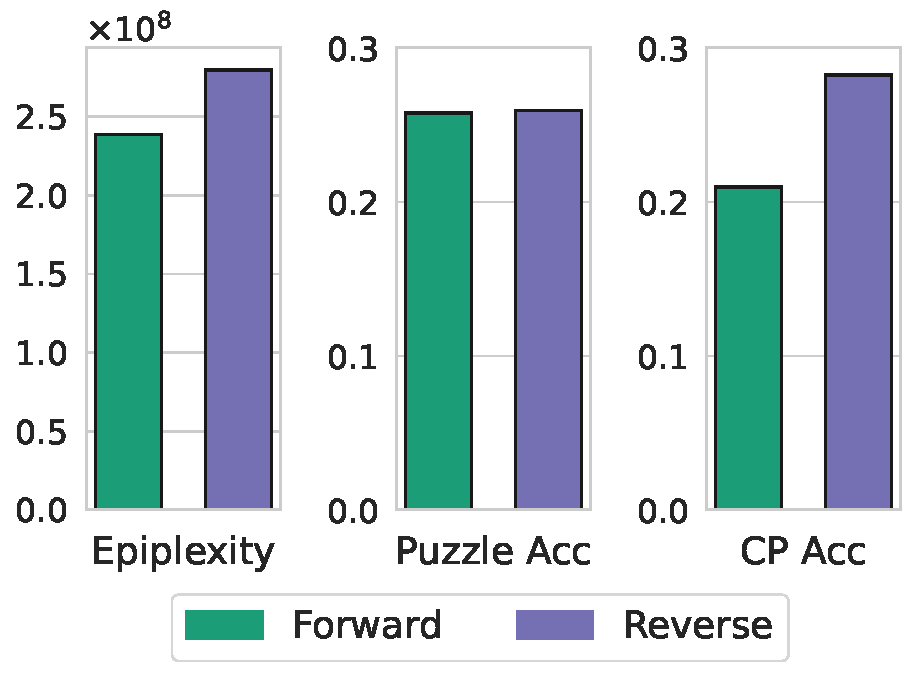
\includegraphics[height=3.0cm]{figs/chess_metrics_bar.pdf}
\end{column}
\end{columns}
\src{Left: $H_T$ and $S_T$ against compute in FLOPs. Right: $S_T$ and accuracy after fine-tuning. Source: Figs.~4c and~7 of \citet{finzi2026}.}
\begin{itemize}
\item At large compute, reverse order gives higher $H_T$ and $S_T$.
\item It transfers better to board evaluation: $0.28$ vs $0.21$ accuracy; puzzles are tied.
\end{itemize}
\take{The reverse order forces a model of the board state. That structure transfers to a task on board states.}
\end{frame}
% ------------------------------------------------------------
\begin{frame}{Application: structure in natural data}
\small
\textbf{Setting.} Equal token budgets and a shared compute bound. Compare OpenWebText, chess and CIFAR-5M with the requential code.

\smallskip
\begin{columns}[T]
\begin{column}{0.38\textwidth}
\centering
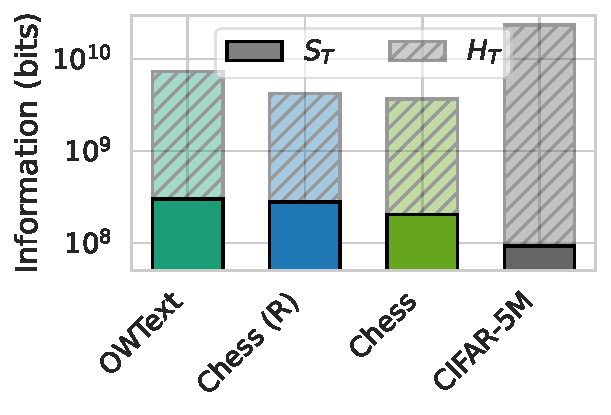
\includegraphics[height=3.3cm]{figs/natural_epi_stacked.pdf}\par
\raggedright
\src{Chess (R): reverse order. Source: Fig.~8a of \citet{finzi2026}. Table: our estimates from the figure.}
\end{column}
\begin{column}{0.58\textwidth}
\begin{tabular}{@{}lccc@{}}
\toprule
Dataset & $S_T$, bits & $\MDL_T$, bits & $S_T/\MDL_T$ \\
\midrule
OpenWebText & $3\times10^8$ & $7\times10^9$ & $4\%$ \\
Chess, reverse & $2.8\times10^8$ & $4\times10^9$ & $7\%$ \\
Chess, forward & $2\times10^8$ & $3.5\times10^9$ & $6\%$ \\
CIFAR-5M & $9\times10^7$ & $2.3\times10^{10}$ & $0.4\%$ \\
\bottomrule
\end{tabular}

\smallskip
\begin{itemize}\setlength{\itemsep}{0.2em}
\item Under this protocol, text has the largest estimated model part; pixel images have the largest residual part.
\item Scaling laws and adaptive data selection show the same ordering \citep{jiang2025}.
\end{itemize}
\end{column}
\end{columns}
\take{This ranking is relative to the tokenisation, model family and compute budget.}
\end{frame}
% ============================================================ SUMMARY
\begin{frame}{Summary and limitations}
\textbf{Summary}
\begin{itemize}\setlength{\itemsep}{0.3em}
\item $S_T$ counts selected model bits; $H_T$ is the expected data-code length.
\item A time bound makes computation, prediction order and learned structure observable.
\item Estimate $S_T$ with prequential area or teacher--student divergence at the compute-optimal model.
\end{itemize}
\medskip
\textbf{Limitations}
\begin{itemize}\setlength{\itemsep}{0.3em}
\item $S_T$ is not a guarantee of downstream usefulness.
\item The theorems are asymptotic and cryptographic; the proved lower bound is only $\Omega(\log n)$.
\item Estimates depend on architecture, optimiser, $T$, dataset size and random seed.
\end{itemize}
\end{frame}
% ============================================================ LITERATURE
\begin{frame}[t]{Literature}
\scriptsize
\begin{thebibliography}{6}\setlength{\itemsep}{0.2em}
\bibitem[Finzi et al.(2026)]{finzi2026}
M.~Finzi et al.\ \emph{From Entropy to Epiplexity}. arXiv:2601.03220v2, 2026.
\bibitem[Qiu et al.(2026)]{qiu2026}
S.~Qiu et al.\ \emph{Requential Coding}. arXiv:2607.11883, 2026.
\bibitem[Li and Vit\'anyi(2008)]{livitanyi2008}
M.~Li, P.~Vit\'anyi.\ \emph{Kolmogorov Complexity}. Springer, 2008.
\bibitem[Wolfram(2002)]{wolfram2002}
S.~Wolfram.\ \emph{A New Kind of Science}. 2002.
\bibitem[Jiang et al.(2025)]{jiang2025}
Y.~Jiang et al.\ Adaptive data optimization.\ \emph{ICLR}, 2025.
\end{thebibliography}
\end{frame}
% ============================================================ QUESTIONS
\begin{frame}{Questions for the audience: answers}
\small
\begin{enumerate}\setlength{\itemsep}{1.1em}
\item A dataset $X$ consists of $n$ uniformly random bits. Which quantity is close to $n$?
\begin{block}{Answer}
$H_T(X)\approx n$: the bounded observer cannot predict the bits. A constant-size uniform model gives $S_T(X)=O(1)$.
\end{block}
\item In the prequential estimate, which part of the training-loss curve approximates the epiplexity?
\begin{block}{Answer}
The area between the loss before each update and the final-model loss, namely
$\sum_i[\log 1/P_i(Z_i)-\log 1/P_M(Z_i)]$.
\end{block}
\item What does changing $T$ change?
\begin{block}{Answer}
It changes the available observer. The total $\MDL_T$ cannot increase with $T$, while $S_T$ itself may rise or fall.
\end{block}
\end{enumerate}
\end{frame}
% ============================================================ BACKUP
\begin{frame}{Backup: basic properties}
\begin{proposition}[Sec.~3 of the paper]
Let $c_1,c_2$ be constants independent of $X$. For a random variable $X$ on $\{0,1\}^n$:
\begin{enumerate}
\item $S_T(X)\ge0$ and $H_T(X)\ge0$;
\item $H(X)\le\MDL_T(X)\le n+c_1$;
\item $\MDL_{T'}(X)\le\MDL_T(X)$ whenever $T'(n)\ge T(n)$;
\item $\MDL_{T'}(f^{-1}(X))\le\MDL_T(X)+|\mathrm f|+c_2$ with $T'(n)=T(n)+\mathrm{Time}(\mathrm f)$, for a program $\mathrm f$ that computes a bijection $f$ in fixed time.
\end{enumerate}
\end{proposition}
Property~4 is the analogue of $K(f(x))\le K(x)+K(f)+c$. Under a time bound a short program for $f^{-1}$ gives no short program for $f$.
\begin{theorem}[Thm.~10 of the paper]
If one-way functions secure against probabilistic polynomial-time algorithms with polynomial advice exist, then some random variables $X_n$ on $\{0,1\}^n$ have $S_{\Poly}(X_n)=\Omega(\log n)$.
\end{theorem}
\end{frame}
% ------------------------------------------------------------
\begin{frame}{Backup: emergence, where $S_T$ falls as $T$ grows}
\begin{columns}[T]
\begin{column}{0.52\textwidth}
\small
\textbf{Setting.} ECA rule~54, $64$ updates. A non-looped transformer predicts the final state directly. A looped transformer generates the intermediate states one after another: the exact simulation.

\medskip
\begin{itemize}\setlength{\itemsep}{0.4em}
\item Below $10^{15}$ FLOPs the non-looped model gives the shorter code. The epiplexity of this model rises to $1.45\times10^7$ bits: it learns emergent patterns of rule~54.
\item Above that bound the looped model gives the shorter code. $\MDL_T$ drops to almost zero; $S_T$ falls.
\item The authors call this case uncommon. For natural data at moderate compute they expect $S_T$ to grow with compute.
\end{itemize}
\end{column}
\begin{column}{0.44\textwidth}
\centering
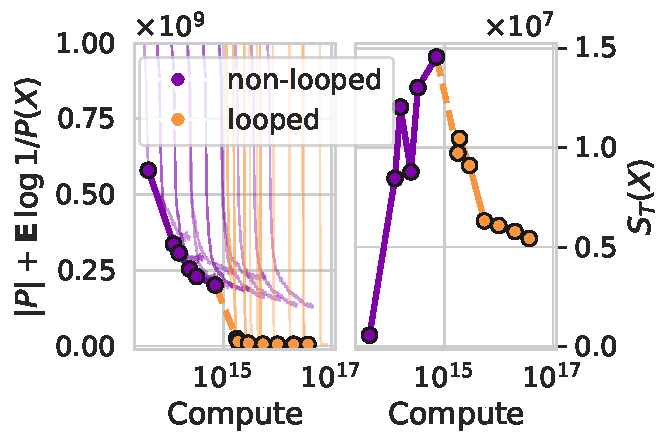
\includegraphics[width=\linewidth]{figs/eca_emergence.pdf}
\raggedright
\src{Two-part code and $S_T$ against compute in FLOPs. Source: Fig.~6 of \citet{finzi2026}.}
\end{column}
\end{columns}
\take{With less compute the best model is a longer program: $S_T$ need not grow with $T$.}
\end{frame}
\end{document}
